\documentclass[10pt]{article} 
\usepackage{ctex}
\usepackage{graphicx}
\usepackage{amsmath}
\usepackage{epstopdf}
\usepackage{tabularx}
\usepackage{geometry}
\usepackage{float}
\usepackage{listings}
\usepackage{xcolor}
\usepackage{fontspec}
\usepackage{color}
\geometry{right=1cm,left=1cm,top=1cm,bottom=1.5cm}
\definecolor{vgreen}{RGB}{104,180,104}
\definecolor{vblue}{RGB}{49,49,255}
\definecolor{vorange}{RGB}{255,143,102}
\lstdefinestyle{verilog-style}
{
    language=Verilog,
    basicstyle=\small\ttfamily,
    keywordstyle=\color{vblue},
    identifierstyle=\color{vblue},
    commentstyle=\color{vgreen},
    numbers=left,
    numberstyle=\tiny\color{black},
    numbersep=10pt,
    tabsize=8,
    moredelim=*[s][\colorIndex]{[}{]},
    literate=*{:}{:}1
}
\makeatletter
\newcommand*\@lbracket{[}
\newcommand*\@rbracket{]}
\newcommand*\@colon{:}
\newcommand*\colorIndex{%
    \edef\@temp{\the\lst@token}%
    \ifx\@temp\@lbracket \color{black}%
    \else\ifx\@temp\@rbracket \color{black}%
    \else\ifx\@temp\@colon \color{black}%
    \else \color{vorange}%
    \fi\fi\fi
}
\makeatother
\usepackage{trace}
\title{流水线设计大作业}
\author{王炜致\ 2022010542}
\date{}
\begin{document}
\maketitle
\tableofcontents
\section{实验目的}
通过将单周期处理器改造为流水线处理器的实践操作,
深刻领会并巩固《数字逻辑与处理器基础》课程中
所学处理器相关知识,
重点掌握汇编指令、冒险处理、外设等的架构与设计,
提高汇编语言及verilog硬件描述语言的理解与编程能力,
体会处理器的设计及优化升级过程。

\section{设计方案及设计过程(含仿真情况与关键代码)}
\subsection{总体设计}
该流水线为经典的五级流水线,由《数字逻辑与处理器基础》课程中提供的单周期处理器
改造而来;此外,还沿用了理论课中编写的排序代码。
这两块基石的基本原理,在此不再赘述,以下展示的是利用
单周期处理器运行排序代码的仿真结果,旨在证明单周期处理器代码
及排序代码(为适配处理器,略有修改)的可靠性:

\begin{figure}[H]
    \centering
    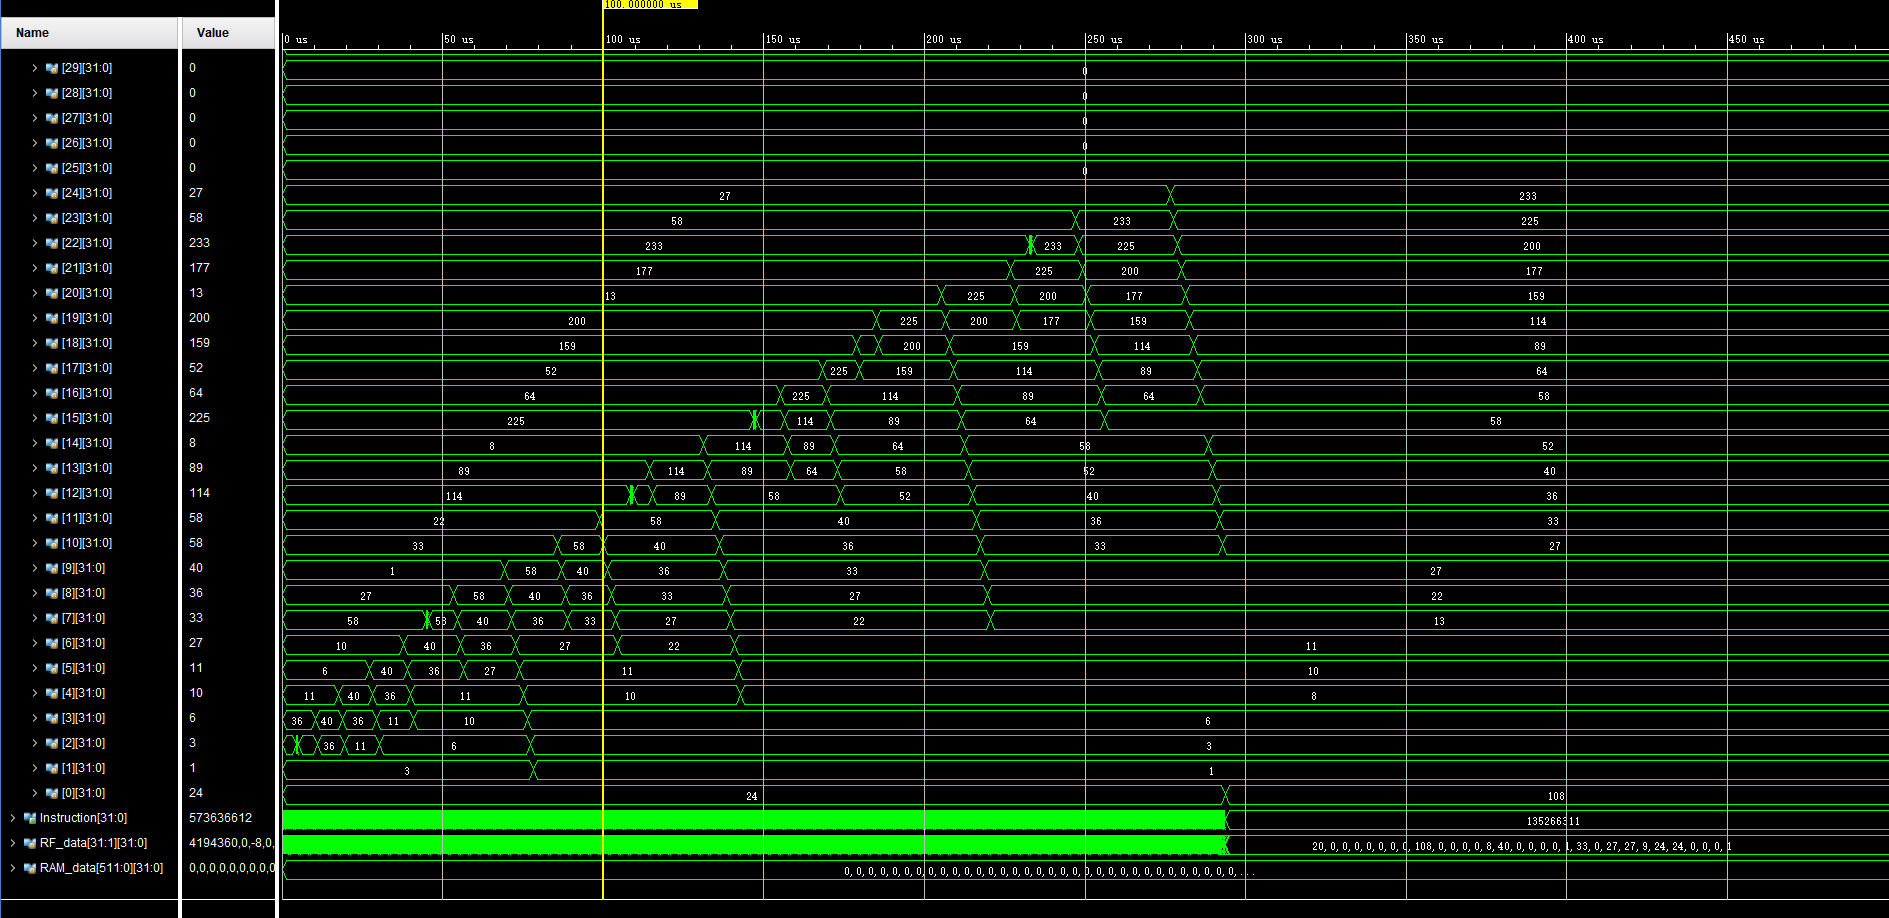
\includegraphics[scale=0.35]{MUCHOGUSTO.png}
    \caption{单周期处理器运行插入排序代码}
    \end{figure}

在改造的过程中,我在CPU.v模块中划分IF,ID,EX,MEM,WB五个阶段,
在阶段之间插入IFID,IDEX,EXMEM,MEMWB四个寄存器堆以服务于数据
转发等功能(详见“冒险处理设计”一节),这也是改造的主体部分;
此外,为扩充指令集,Control.v需要扩展或调整Branch等信号(Branch[2:0]);
为实现数据初始化及配合软件控制,DataMemory.v也需要接受一定的改造与扩展;
为在特定处理器条件下适应处理器局限性、执行给定的任务,
汇编代码也需要经过修订与增补,再写入InstructionMemory.v中。

该流水线处理器的实现历时约五天(7.1-7.5)。预估到工作量庞大,
为避免后期debug困难,我遵循小心谨慎、勤做仿真、步步为营的工作方针,
因而总体设计历程层次分明:验证单周期处理器及代码可靠性、扩充指令集、插入
寄存器堆(不考虑冒险)、处理结构冒险、处理数据冒险、处理控制冒险,到此先
使用译码器方法上板验证,硬件调试成功后,再使用软件方法完成了实验。除串口
部分外,实验内容均已完成并提前约2周通过验收。设计历程有存档,可以在附录文件中
查看。

以下展示的是流水线处理器设计总框图,为使画面简明扼要,
略去不画MUX,Forwarding,Jump,Branch单元的控制信号。相关信息将在下文具体介绍。
由图可见,IF阶段主要执行取指令及生成控制信号操作;ID阶段主要执行后序指令的判断与跳转
、生成ALU控制信号、读取寄存器堆操作;EX阶段主要进行ALU运算操作;MEM阶段主要进行
读写存储器堆及控制外设(BCD)操作;WB阶段主要进行写回操作。
\begin{figure}[H]
    \centering
    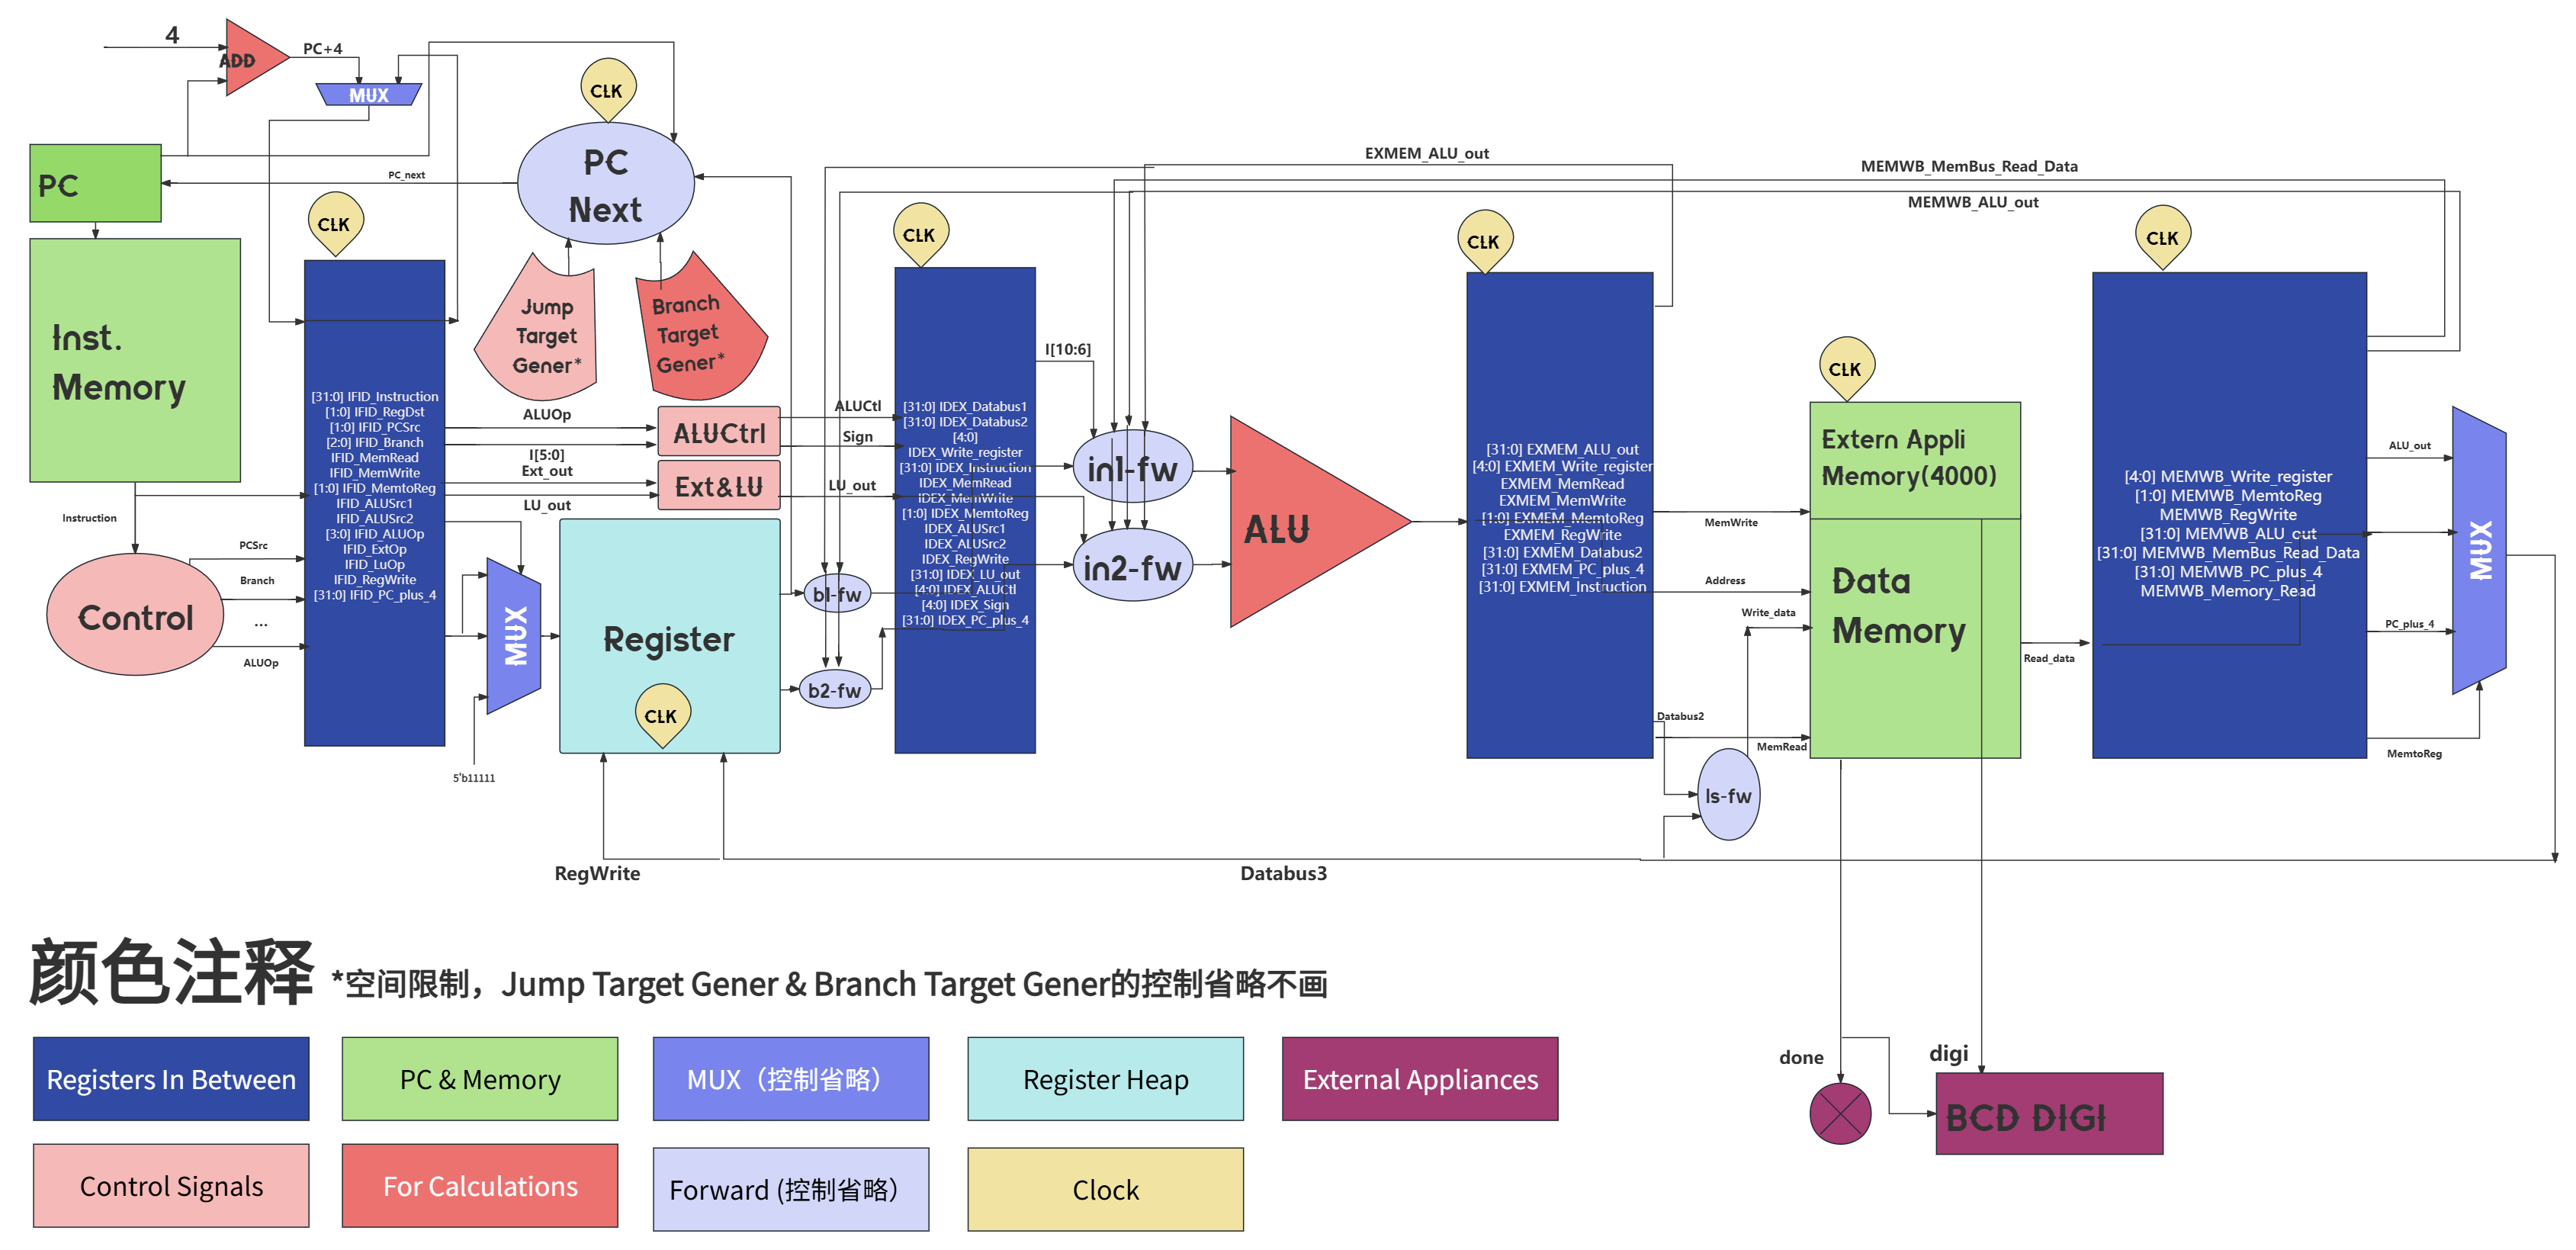
\includegraphics[scale=0.163]{panor.png}
    \caption{流水线处理器设计框图(有省略)}
    \end{figure}
\subsection{指令集扩充设计}
根据指导书要求,参阅MIPS文档,扩充跳转与分支指令如下:
\begin{table}[h]
    \footnotesize
\begin{center}
    \begin{tabular}{|r|r|r|r|r|r|r|r|r|r|r|r|}
        \hline
        &PCSrc[1:0]& Branch & RegWrite & RegDst[1:0] & MemRead & MemWrite & MemtoReg[1:0] & ALUSrc2 & ALUSrc1 & ExtOp & LuOp\\
        \hline
        bne & 0(00) & 1 & 0 & x(xx) & x & 0 & x(xx) & 0 & 0 & 1 & x\\
        \hline
        blez& 0(00) & 1 & 0 & x(xx) & x & 0 & x(xx) & 0 & 0 & 1 & x\\
        \hline
        bgtz& 0(00) & 1 & 0 & x(xx) & x & 0 & x(xx) & 0 & 0 & 1 & x\\
        \hline
        bltz& 0(00) & 1 & 0 & x(xx) & x & 0 & x(xx) & 0 & 0 & 1 & x\\
        \hline
        jalr& 2(10) & x & 1 & 1(01) & x & 0 & 2(10) & x & x & x & x\\
        \hline
    \end{tabular}
\end{center}
\end{table}

相应地修改了控制信号生成模块Control.v及模块端口,详见所附源代码。

\subsection{测试数据设计}
设置数据内存大小为256个字。按要求,准备24个待排序正整数,
在DataMemory.v中初始化RAMdata[1:24],作为测试样例。RAMdata[0]
存储的是待排序正整数的数量。

\begin{lstlisting}[style={verilog-style}]
    //DataMemory.v
    parameter RAM_SIZE = 512;
    parameter RAM_SIZE_BIT = 8;
    reg [31:0] RAM_data [RAM_SIZE - 1: 0];
    ...
    if (reset) begin
            RAM_data[0] <= 32'h00000018; //numbers=24
            
            RAM_data[1] <= 32'h00000003; 
            RAM_data[2] <= 32'h00000028; 
            RAM_data[3] <= 32'h00000024; 
            RAM_data[4] <= 32'h0000020B; 
            RAM_data[5] <= 32'h00003406; 
            RAM_data[6] <= 32'h00000A0A; 
            RAM_data[7] <= 32'h0000F03A; 
            RAM_data[8] <= 32'h0000001B; 
            
            RAM_data[9] <= 32'h00000001; 
            RAM_data[10] <= 32'h00009021; 
            RAM_data[11] <= 32'h00000216; 
            RAM_data[12] <= 32'h00000072; 
            RAM_data[13] <= 32'h00000059; 
            RAM_data[14] <= 32'h00000007; 
            RAM_data[15] <= 32'h000003E1; 
            RAM_data[16] <= 32'h00000B40; 
            
            RAM_data[17] <= 32'h00000034; 
            RAM_data[18] <= 32'h0000009F; 
            RAM_data[19] <= 32'h000000C8;
            RAM_data[20] <= 32'h0000000D; 
            RAM_data[21] <= 32'h000000B1; 
            RAM_data[22] <= 32'h000000E9; 
            RAM_data[23] <= 32'h0000003a; 
            RAM_data[24] <= 32'h0000001B; 
        
            for (i = 25; i < RAM_SIZE; i = i + 1)
                RAM_data[i] <= 32'h00000000;
\end{lstlisting}

排序部分使用《数字逻辑与处理器基础》课程中设计的插入排序算法,详见所附源代码。排序
完成后,

\subsection{冒险处理设计}
\subsubsection{结构冒险}
在前述框图中,InstructionMemory与DataMemory已作分离;R型指令
Mem阶段已空置;ALU已作功能疏解。结构冒险已经得到解决。
\subsubsection{数据冒险}
\underline{\large 同时读写寄存器堆}
\begin{figure}[H]
    \centering
    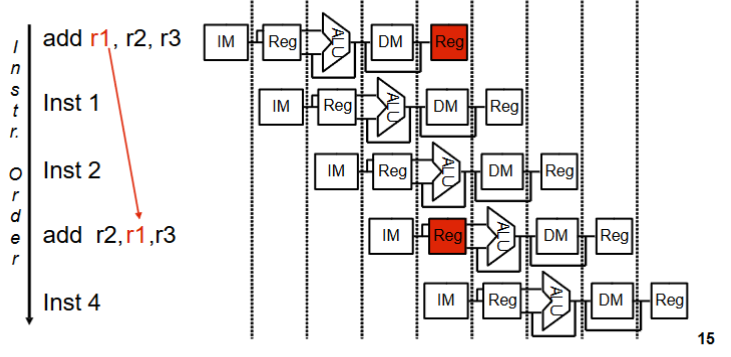
\includegraphics[scale=0.4]{reguse.png}
    \caption{数据冒险之同时读写寄存器堆}
    \end{figure}

根据理论所学,应通过先写后读策略处理:
\begin{lstlisting}[style={verilog-style}]
    //RegisterFile.v
    always @(*) begin
        if (RegWrite && (Write_register != 5'b00000))
             RF_data[Write_register] = Write_data;//first write
        Read_data1 = (Read_register1 == 5'b00000)? 32'h00000000: RF_data[Read_register1];
        Read_data2 = (Read_register2 == 5'b00000)? 32'h00000000: RF_data[Read_register2];
    end
\end{lstlisting}
验证如下:
\begin{figure}[H]
    \centering
    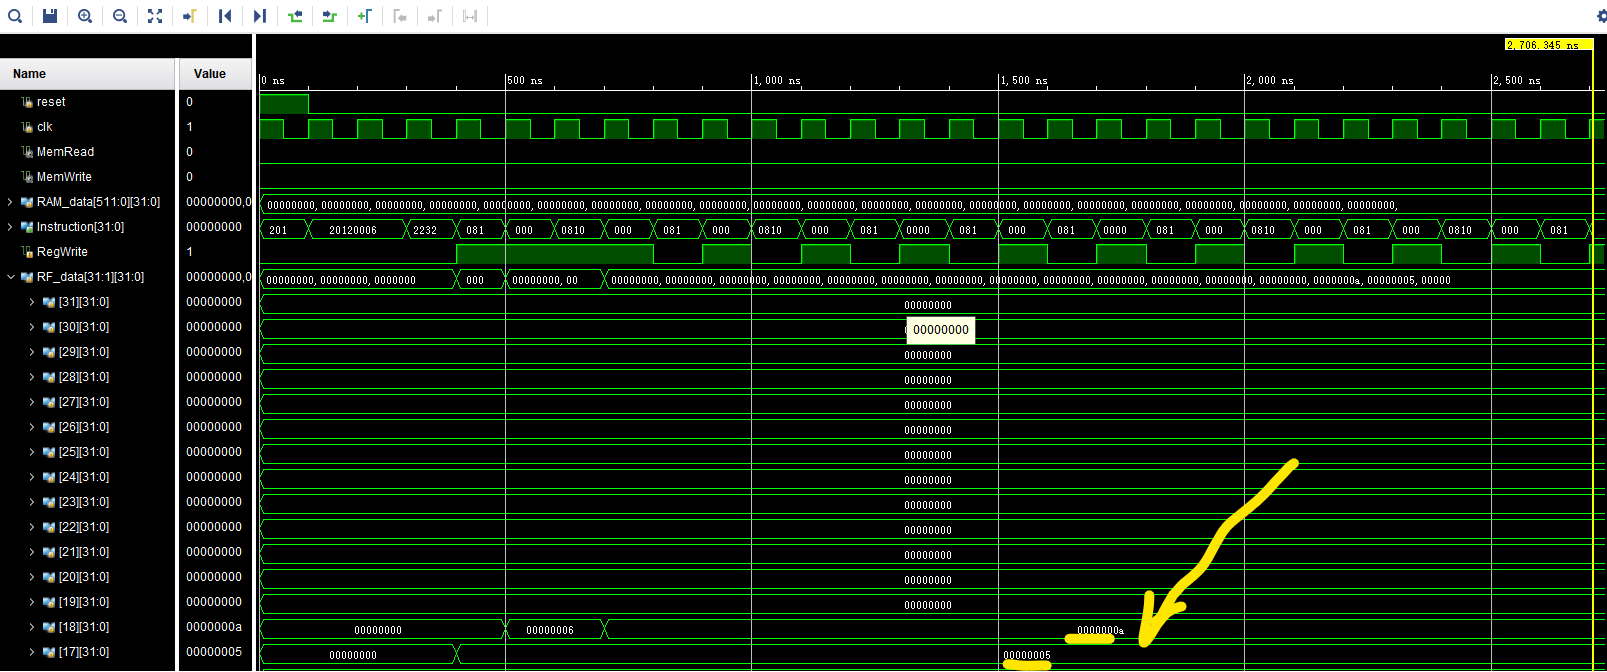
\includegraphics[scale=0.43]{fwtr.png}
    \caption{先写后读前仿验证}
    \end{figure}
    \begin{figure}[H]
        \centering
        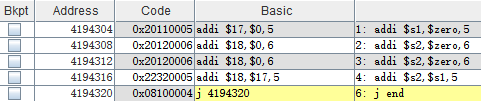
\includegraphics[scale=0.9]{fwtrx.png}
        \caption{先写后读验证测试代码}
        \end{figure}
但在布线过程中发现always块内阻塞赋值会报错,故后期改为转发实现。

\underline{\large 时间顺序关联(ALU输出)}

对于R型指令,ALU输出运算结果后尚未写回寄存器堆,
而后序指令可能需要使用新数据,故应转发给ALU输入端。
需要修改ALU的输入端(二路),增加MUX选择合适的输入信号:
\begin{figure}[H]
    \centering
    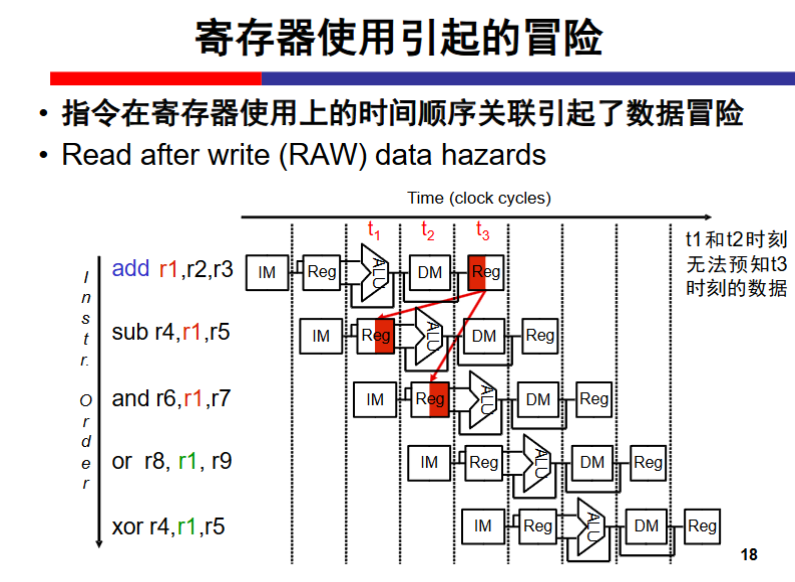
\includegraphics[scale=0.3]{reg.png}
    \caption{数据冒险之ALU输出}
    \end{figure}

\begin{lstlisting}[style={verilog-style}]
    //CPU.v
    wire [32 -1:0] in1,in2;//rs,rt forwarding
    assign in1 = (~IDEX_ALUSrc1 && MEMWB_Memory_Read && MEMWB_Write_register 
        && MEMWB_Write_register == IDEX_Instruction[25:21])? MEMWB_MemBus_Read_Data:
        (~IDEX_ALUSrc1 && MEMWB_RegWrite && MEMWB_Write_register && 
        (MEMWB_Write_register == IDEX_Instruction[25:21])
        && (EXMEM_Write_register != IDEX_Instruction[25:21] || ~EXMEM_RegWrite))? 
        MEMWB_ALU_out:
        (~IDEX_ALUSrc1 && EXMEM_RegWrite && EXMEM_Write_register
        && (EXMEM_Write_register == IDEX_Instruction[25:21]))? EXMEM_ALU_out: 
        ALU_in1;
    assign in2 = (~IDEX_ALUSrc2 && MEMWB_Memory_Read && MEMWB_Write_register 
        && MEMWB_Write_register == IDEX_Instruction[20:16])? MEMWB_MemBus_Read_Data:
        (~IDEX_ALUSrc2 && MEMWB_RegWrite && MEMWB_Write_register && 
        (MEMWB_Write_register == IDEX_Instruction[20:16])
        && (EXMEM_Write_register != IDEX_Instruction[20:16] || ~EXMEM_RegWrite))? 
        MEMWB_ALU_out://mind load-store
        (~IDEX_ALUSrc2 && EXMEM_RegWrite && EXMEM_Write_register
        && (EXMEM_Write_register == IDEX_Instruction[20:16]))? EXMEM_ALU_out: 
        ALU_in2;
\end{lstlisting}
验证如下(汇编代码及其对应的仿真结果):
\begin{figure}[H]
    \centering
    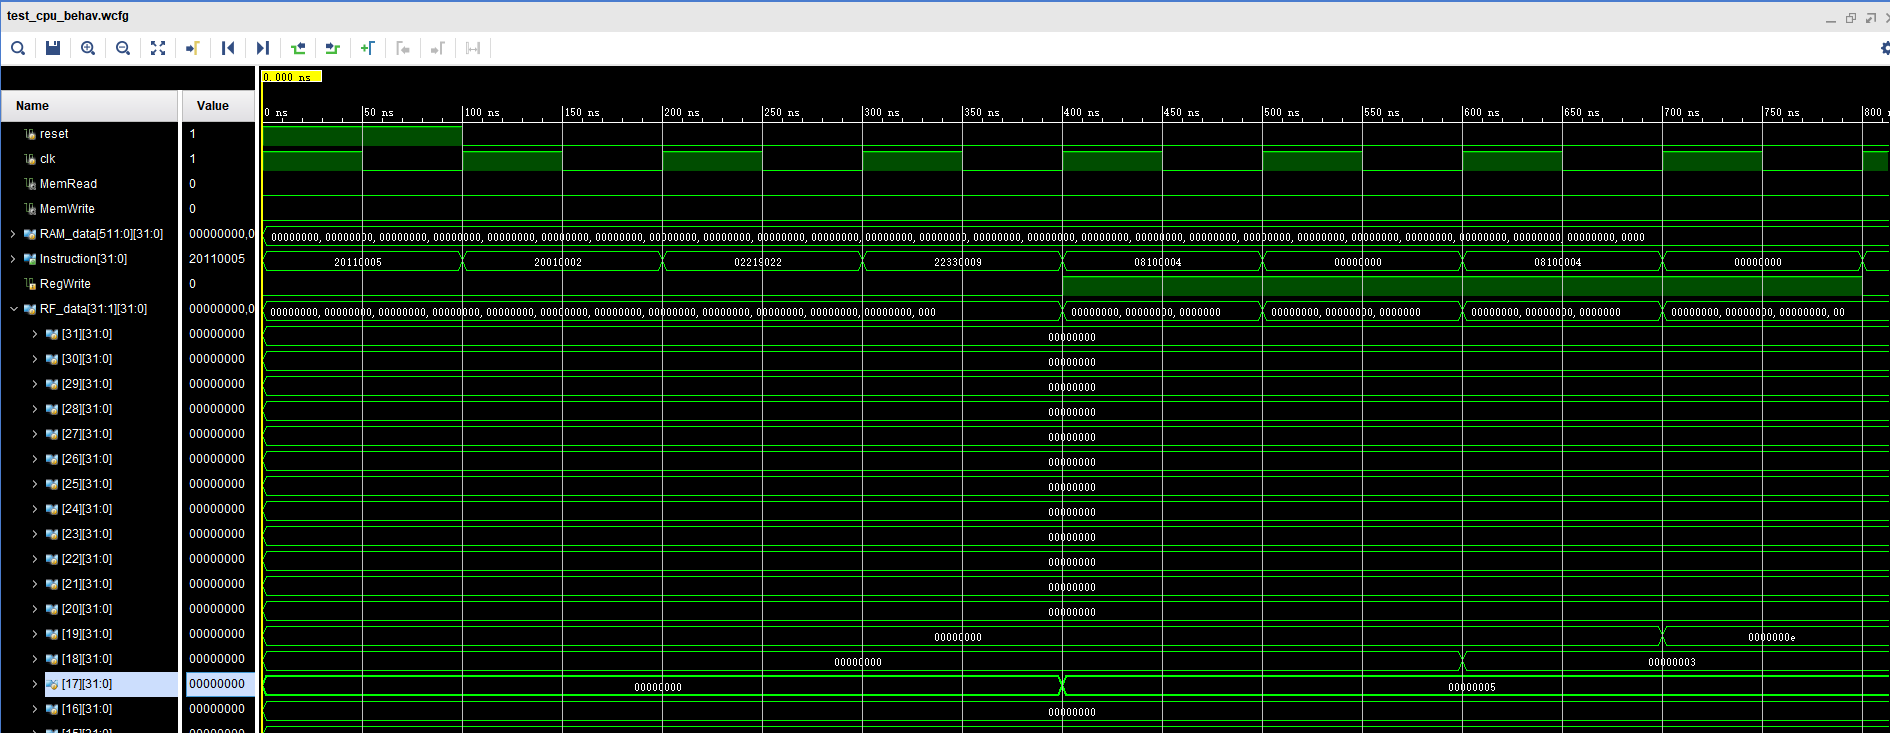
\includegraphics[scale=0.35]{haddaz.png}
    \caption{数据转发前仿验证}
    \end{figure}
    \begin{figure}[H]
        \centering
        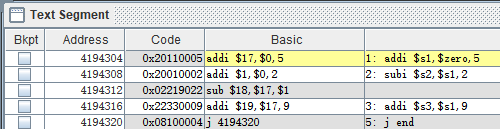
\includegraphics[scale=0.9]{hadd.png}
        \caption{数据转发验证测试代码}
        \end{figure}
此外,若下一条指令为Branch(为简便,默认jr,jalr使用\$31,故不需要处理),
则不能不stall一个周期,再将数据转发到ID阶段:
\begin{lstlisting}[style={verilog-style}]
    //CPU.v
    assign Databus1_brc = (MEMWB_Write_register && MEMWB_RegWrite
        && MEMWB_Write_register == IFID_Instruction[25:21] && 
        (EXMEM_Write_register != IFID_Instruction[25:21] || ~EXMEM_RegWrite))? MEMWB_ALU_out:
        (EXMEM_Write_register && EXMEM_RegWrite
        && EXMEM_Write_register == IFID_Instruction[25:21])? EXMEM_ALU_out:
        Databus1;
    assign Databus2_brc = (MEMWB_Write_register && MEMWB_RegWrite
        && MEMWB_Write_register == IFID_Instruction[20:16] &&
         (EXMEM_Write_register != IFID_Instruction[20:16] || ~EXMEM_RegWrite))? MEMWB_ALU_out:
        (EXMEM_Write_register && EXMEM_RegWrite
        && EXMEM_Write_register == IFID_Instruction[20:16])? EXMEM_ALU_out:
        Databus2;
\end{lstlisting}

验证如下(汇编代码及其对应的仿真结果):
\begin{figure}[H]
    \centering
    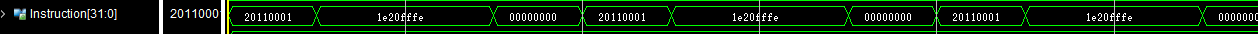
\includegraphics[scale=0.4]{bgtzz.png}
    \caption{Branch指令前自带stall前仿验证}
    \end{figure}
    \begin{figure}[H]
        \centering
        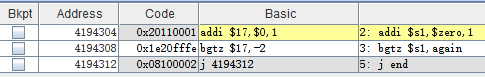
\includegraphics[scale=0.9]{bgtz.png}
        \caption{Branch指令前自带stall验证测试代码}
        \end{figure}
\subsubsection{load-use冒险}
\begin{figure}[H]
    \centering
    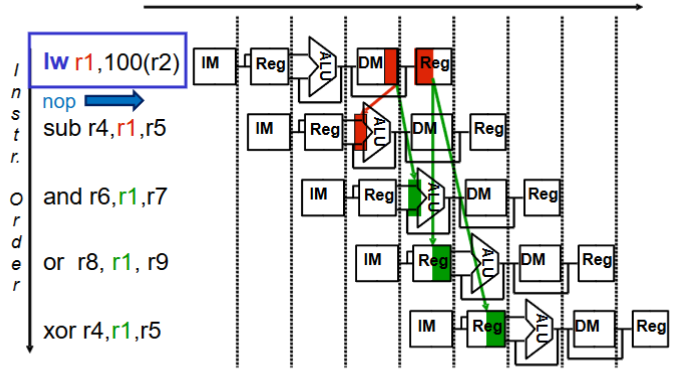
\includegraphics[scale=0.6]{load.png}
    \caption{load-use冒险}
    \end{figure}
load-use冒险包含load-R类和load-store类冒险,前者不可避免地需要stall一个周期。
故需要将读出数据作转发。
处理load-store冒险时,在ALU输入forwarding条件中需要分辨立即数加法与寄存值加法;
DataMemory写端口也需要forwarding判断:
\begin{lstlisting}[style={verilog-style}]
    //CPU.v
    assign MemBus_Write_Data  = (Memory_Write && MEMWB_Write_register 
	                        && (MEMWB_Write_register == EXMEM_Instruction[20:16]))? Databus3
	                        :EXMEM_Databus2;//for load-store special case:lw s1,x;sw s1,s1
\end{lstlisting}
在仿真测试时发现一种非常特殊的情况——形如
lw \$s1,4(\$zero),sw \$s1,0(\$s1)——由于stall一个周期,无法由MEM/WB转发,同时\$s1尚未
更新。故需要特殊处理:
\begin{lstlisting}[style={verilog-style}]
    //CPU.v
    wire [32 -1:0] IDEX_Databus2_prevent_loadstore;
    assign IDEX_Databus2_prevent_loadstore = (IDEX_MemWrite && MEMWB_Write_register
        && (MEMWB_Write_register == IDEX_Instruction[20:16]))? MEMWB_MemBus_Read_Data:
        IDEX_Databus2;
\end{lstlisting}
一般load-use处理效果如下(汇编代码及其对应的仿真结果):
\begin{figure}[H]
    \centering
    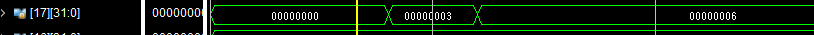
\includegraphics[scale=0.6]{add.png}
    \caption{load-use处理前仿验证}
    \end{figure}
    \begin{figure}[H]
        \centering
        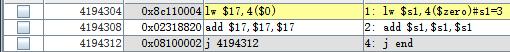
\includegraphics[scale=0.9]{addon.png}
        \caption{load-use处理验证测试代码}
        \end{figure}
一般load-store处理效果如下(汇编代码及其对应的仿真结果):
\begin{figure}[H]
    \centering
    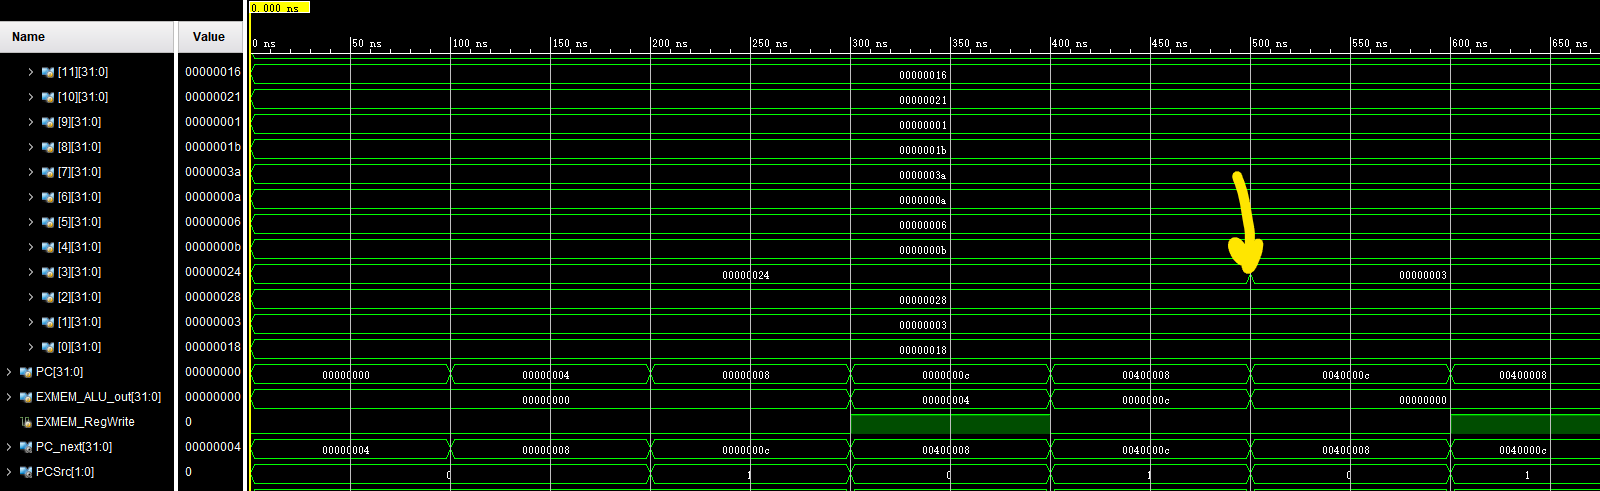
\includegraphics[scale=0.4]{lstore.png}
    \caption{load-store处理前仿验证}
    \end{figure}
    \begin{figure}[H]
        \centering
        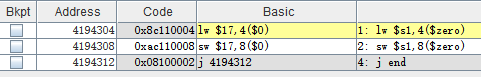
\includegraphics[scale=0.9]{fo.png}
        \caption{load-store处理验证测试代码}
        \end{figure}
特殊load-store处理效果如下(汇编代码及其对应的仿真结果):
\begin{figure}[H]
    \centering
    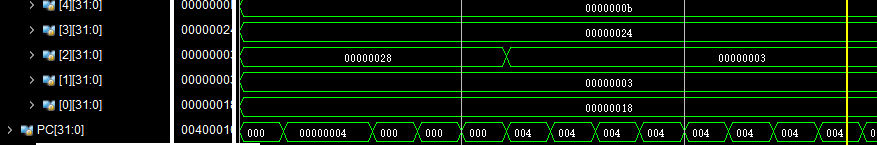
\includegraphics[scale=0.5]{specialls.png}
    \caption{特殊load-store处理验证测试代码}
    \end{figure}
\begin{figure}[H]
    \centering
    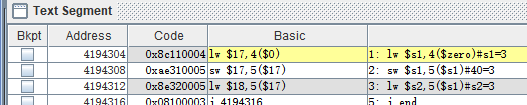
\includegraphics[scale=0.9]{hdl.png}
    \caption{特殊load-store处理验证测试代码}
    \end{figure}

另外,load后若紧跟Branch指令且发生冒险,则需要stall两个周期,
在此不作处理,通过在汇编代码中添加3个nop指令(0x00000000)解决。
至此,数据冒险基本解决。
\subsubsection{控制冒险}
由于提前到ID阶段进行新指令相关操作,接下来执行哪条指令需要等待两个周期才能出结果。故
设定Branch、Jump指令下一条指令必为nop,即等待一个周期,这样能够比较方便地规避控制冒险。

处理完上述冒险后,利用流水线处理器排序结果仿真如下,可见排序已能正确实现:
\begin{figure}[H]
    \centering
    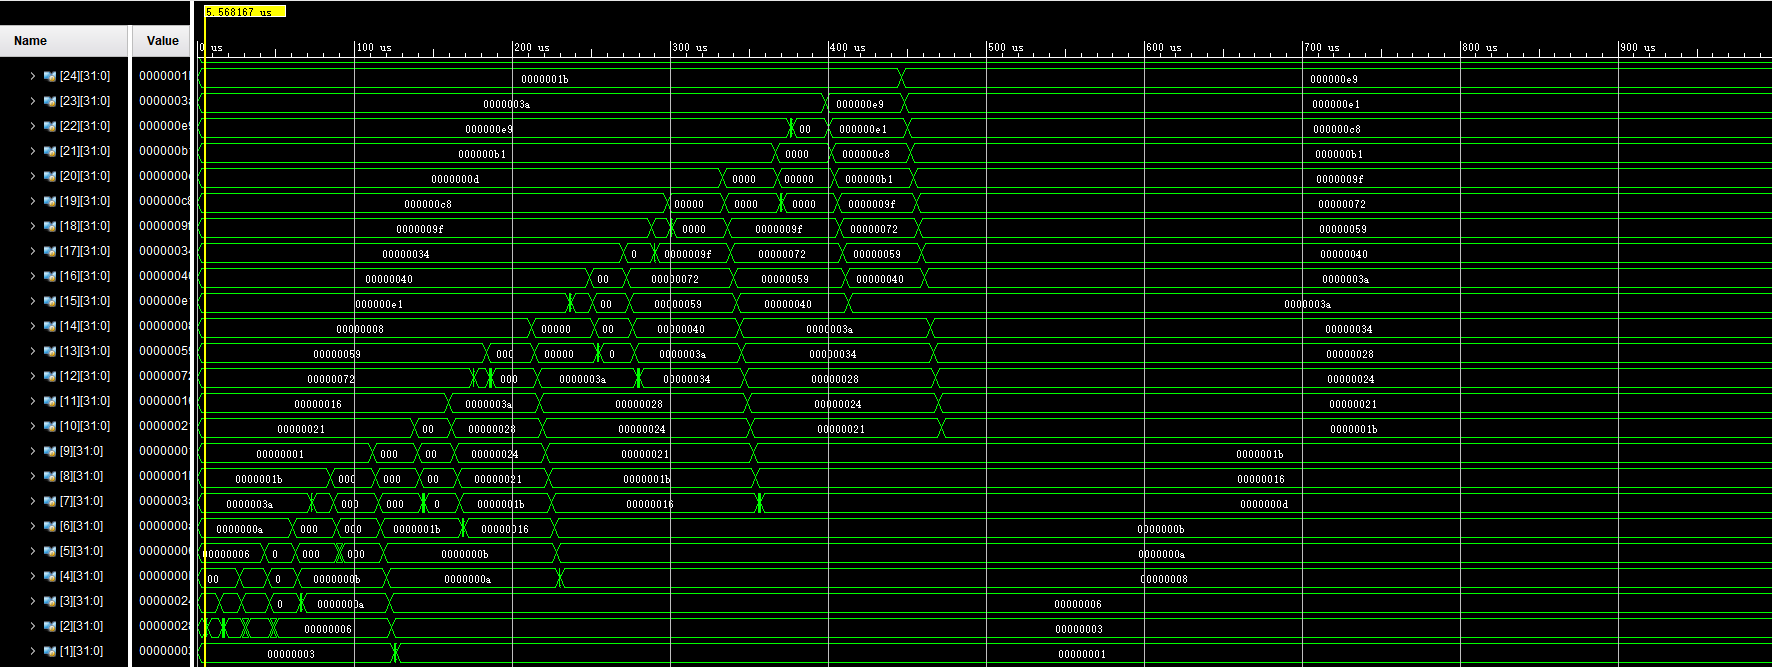
\includegraphics[scale=0.37]{mult.png}
    \caption{冒险处理后排序效果的前仿验证}
    \end{figure}
\subsection{外设与WELOG实验板行为设计}
\subsubsection{外设设计}
我的流水线外设设计主要参考了PPT中的设计,但也存在一大不同。我的汇编代码中不存在
读取外设存储器的lw指令,verilog代码中也省略了读外设存储器的硬件配套。事实上,
只需要通过“写入外设存储器”的指令来维护外设控制信号,
而“读取外设存储器”的操作,应当是不必要的。让外设存储器直接与外设相连,即直接控制外设,
也能保证功能的正常实现,且更加简捷。

更多相关内容可参阅“算法指令”一节。
\begin{figure}[H]
    \centering
    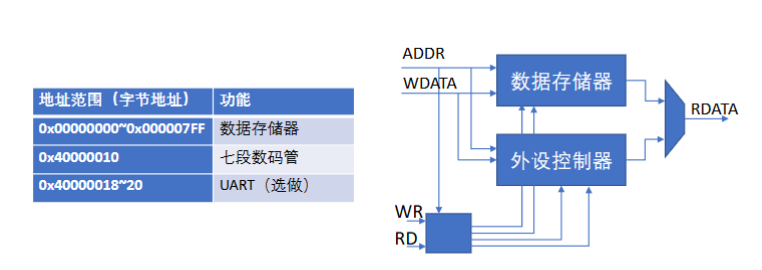
\includegraphics[scale=0.5]{exter.png}
    \caption{PPT提供的外设参考设计}
    \end{figure}
\subsubsection{WELOG实验板行为设计}
排序程序执行完之后,一颗LED将点亮以指示完成排序,此后七段数码管将
从小到大显示用十六进制表示的正整数,每隔1秒切换,无限循环显示。约定
字母按如下规则显示:
\begin{figure}[H]
    \centering
    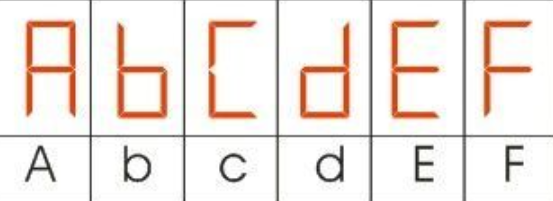
\includegraphics[scale=0.6]{abc.png}
    \caption{十六进制数显示约定}
    \end{figure}
\section{算法指令}
MIPS指令主要分为两个部分:排序功能实现部分以及软件形式数显控制部分。
前者使用插入排序,不再赘述;下面将介绍后者,这段代码在排序代码运行完毕之后
执行:

\begin{lstlisting}[style={verilog-style}]
    #MIPS_Code.asm
    addi $a1,$a1,1
    sll $a1,$a1,2
    addi $s6,$zero,1
    sw $s6,0($a1)
    addi $a1,$a1,4 #saving current sorted data
    
    lui $s0,0x4000
    
    addi $s0,$s0,16 #40000010
    addi $t1,$zero,80 
    
rounding:
   lw $s1,0($a1) #s1 0xabcd,renewed every second
   add $t0,$zero,$zero #zero,count 100000 then break
bcd4:#lowest
   addi $t0,$t0,1
   andi $s2,$s1,0x0000000f #get lowest 4 bits
   jal judging
   addi $s3,$s3,256 #add ano lowest
   sw $s3,0($s0)
   bne $t0,$t1,bcd4
   
   add $t0,$zero,$zero #zero,count 100000 then break
bcd3:	
   addi $t0,$t0,1
   andi $s2,$s1,0x000000f0 #get 2-lowest 4 bits
   srl $s2,$s2,4
   jal judging
   addi $s3,$s3,512
   sw $s3,0($s0)
   bne $t0,$t1,bcd3
   
   add $t0,$zero,$zero #zero,count 100000 then break
bcd2:
   addi $t0,$t0,1
   andi $s2,$s1,0x00000f00 #get 2-highest 4 bits
   srl $s2,$s2,8
   jal judging
   addi $s3,$s3,1024
   sw $s3,0($s0)
   bne $t0,$t1,bcd2
   
   add $t0,$zero,$zero #zero,count 100000 then break
bcd1:	
   addi $t0,$t0,1
   andi $s2,$s1,0x0000f000 #get highest 4 bits
   srl $s2,$s2,12
   jal judging
   addi $s3,$s3,2048 #add ano highest
   sw $s3,0($s0)
   bne $t0,$t1,bcd1
   
   j rounding

judging:
   beq $s2,15,f
   beq $s2,14,e
   beq $s2,13,d
   beq $s2,12,c
   beq $s2,11,B
   beq $s2,10,a
   beq $s2,9,ni
   beq $s2,8,ei
   beq $s2,7,se
   beq $s2,6,si
   beq $s2,5,fi
   beq $s2,4,fo
   beq $s2,3,th
   beq $s2,2,tw
   beq $s2,1,on
   beq $s2,0,ze
   
f:addi $s3,$zero,113 #0111 0001
   jr $ra
e:addi $s3,$zero,121 
   jr $ra
d:addi $s3,$zero,94
   jr $ra
c:addi $s3,$zero,57
   jr $ra
B:addi $s3,$zero,124
   jr $ra
a:addi $s3,$zero,119
   jr $ra
ni:addi $s3,$zero,111
   jr $ra
ei:addi $s3,$zero,127
   jr $ra
se:addi $s3,$zero,7
   jr $ra
si:addi $s3,$zero,125
   jr $ra
fi:addi $s3,$zero,109
   jr $ra
fo:addi $s3,$zero,102
   jr $ra
th:addi $s3,$zero,79
   jr $ra
tw:addi $s3,$zero,91
   jr $ra
on:addi $s3,$zero,6
   jr $ra
ze:addi $s3,$zero,63
   jr $ra
\end{lstlisting}

软件操作过程为:当排序完成后,在紧接正整数序列存储区域的下一单元
存入“1”(即由0变为1),表示排序完成。;“1”的下一个单元则用来存放
当前需要展示的正整数,地址为a1。

接下来进入轮询环节。verilog部分负责控制正整数更新(见下方代码),即每隔1秒在a1地址中存入序列中新的正整数值,
这样汇编代码中s1可以在每次rounding循环中自然地检测并获取数据更新。接着,需要扫描当前正整数的各个数位。通过
andi分别读取正整数在16进制下的4个数位,跳转到judging处作(0-15)的判断,再跳转译码,给出
数码管的控制信号。

\begin{lstlisting}[style={verilog-style}]
//DataMemory.v
reg [16 -1:0] counting;//fetch data
parameter Hz = 100000000;//1s,based on 100MHz
reg [32 -1:0] cHz;//1s timer
always @(posedge reset or posedge clk)begin
	if (reset) begin
            RAM_data[0] <= 32'h00000018; //numbers=24
            ...
            cHz <= 32'h00000000;
            counting <= 16'b1;
            digi <= 12'b0;
	end
	else begin
	    cHz <= (cHz == Hz-32'd1) ? 32'd0 : cHz + 32'd1;
	    if (MemWrite) begin
	        if(Address == 32'h40000010)
		        digi <= Write_data[11:0];//write into digi with address 40000010(sw 40000010)
		    else
			RAM_data[Address[RAM_SIZE_BIT + 1:2]] <= Write_data;
	    end
	    else if (cHz == 32'd0 && done) begin
		    RAM_data[26] <= RAM_data[counting];//address 26 saves the current data
                if (counting < RAM_data[0])
                    counting <= counting+16'b1;
                else
                    counting <= 16'b1;
	    end
	end
end
\end{lstlisting}

DataMemory.v输出控制信号[11:0]digi,与外设相连:
\begin{lstlisting}[style = {verilog-style}]
    wire [11:0] digi;//generate from DMem, designed using mips insts
    assign sel = digi[11:8];//output [3:0]sel
    assign leds = digi[7:0];//output [7:0]leds
\end{lstlisting}
\section{关键代码和文件清单(此处关键代码略)}
提交的文件包含本实验报告和2个文件夹。

CODES文件夹中包含3个源代码文件夹。
其中FINAL\_VERSION\_FOR\_BOARD\_RUNNING
文件夹为专用于上板运行的版本,为确保安全不超频,工作频率为50MHz(用2分频模块处理100MHz
板载时钟),此外还负责资源占用测量;
FINAL\_VERSION\_FOR\_TIMING \& CPI文件夹为测量最高主频的版本,此外还负责CPI测量(仿真
频率为50MHz);SINGLE\_CYCLE文件夹为单周期处理器运行排序算法的版本;HIST
文件夹为历史版本记录,供参考。

PROJECTS文件夹中包含上板运行(onboard)、测量最高主频(pipeline)两个项目版本。

以下是FINAL\_VERSION\_FOR\_BOARD\_RUNNING中的文件:
\begin{table}[h]
    \footnotesize
\begin{center}
    \begin{tabular}{|r|r|}
        \hline
        文件&功能\\
        \hline
        test\_CPU.v&仿真文件\\
        \hline
        CPU.v&CPU主模块,集成了段间寄存器\\
        \hline
        clk\_50M.v&分频得到50MHz安全频率\\
        \hline
        InstructionMemory.v&存储机器语言表示的排序算法\\
        \hline
        Control.v&生成处理器各部件的控制信号\\
        \hline
        RegisterFile.v&寄存器堆\\
        \hline
        ALUControl.v&生成ALU的控制信号\\
        \hline
        ALU.v&计算模块\\
        \hline
        DataMemory.v&数据存储器和外设存储器\\
        \hline
        const.xdc& 管脚约束文件\\
        \hline
        Instructions.txt& 排序算法机器语言代码\\
        \hline
        MIPS\_Code.asm& 排序算法汇编语言代码\\
        \hline
        Mars4\_5.jar& MIPS编译器\\
        \hline
    \end{tabular}
\end{center}
\end{table}

除了一般的verilog文件,FINAL\_VERSION\_FOR\_BOARD\_RUNNING还包括:
\begin{table}[h]
    \footnotesize
\begin{center}
    \begin{tabular}{|r|r|}
        \hline
        文件&功能\\
        \hline
        a.in&输入数据文件\\
        \hline
        gen.cpp&用于生成a.in\\
        \hline
        MIPS\_Code\_CPI.asm&测量指令数用\\
        \hline
    \end{tabular}
\end{center}
\end{table}
\section{综合情况}
\subsection{时序:最高主频}
如图,经过反复测量,发现时钟周期为13.5710ns(Vivado四舍五入为13.5710ns)时,
WNS几乎为0,故可以计算最高时钟频率
$$f_m=\frac{1}{13.5710ns}\approx73.687MHz$$
\begin{figure}[H]
    \centering
    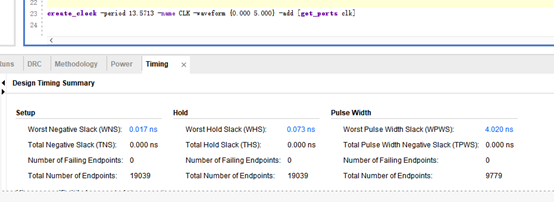
\includegraphics[scale=1]{res.png}
    \caption{测量流水线CPU最高主频(Implementation)}
    \end{figure}
\subsection{面积:资源占用}
\begin{figure}[H]
    \centering
    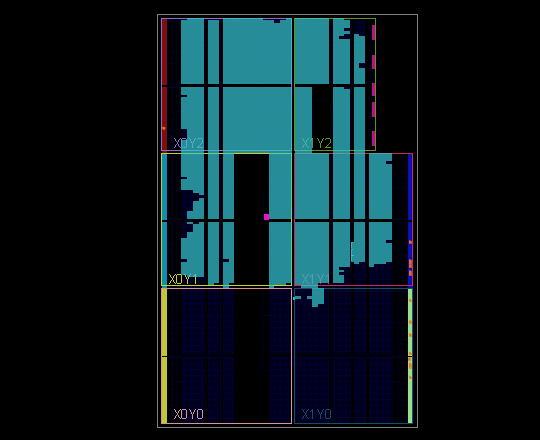
\includegraphics[scale=0.5]{space.png}
    \caption{流水线FPGA面积占用}
    \end{figure}

\begin{figure}[H]
    \centering
    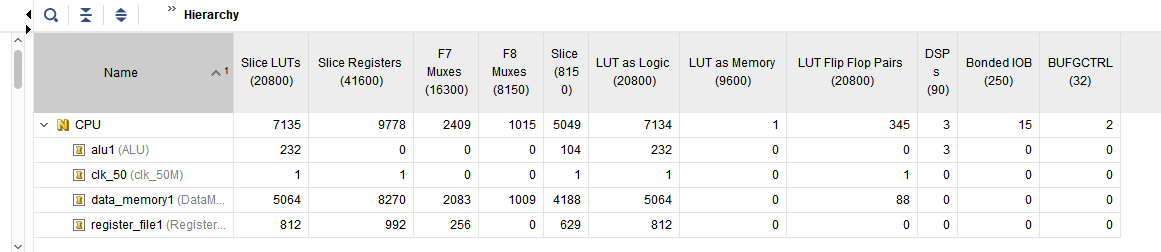
\includegraphics[scale=0.5]{num.png}
    \caption{流水线资源占用数量}
    \end{figure}

\begin{figure}[H]
    \centering
    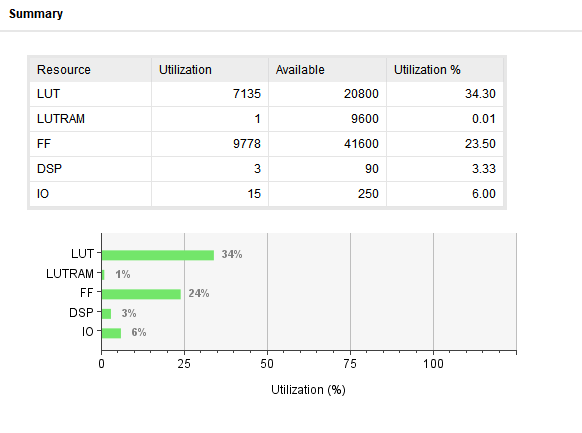
\includegraphics[scale=0.7]{par.png}
    \caption{流水线资源占用比例}
    \end{figure}

可见,LUT的占用率最高,达到34.3\%,存储器占据了大量的查找表资源;
由于寄存器的大量存在,D触发器的占用比例也较高,达到23.50\%。相比
单周期处理器,LUT,FF的使用都有所增加,是资源换时间的体现。

\begin{figure}[H]
    \centering
    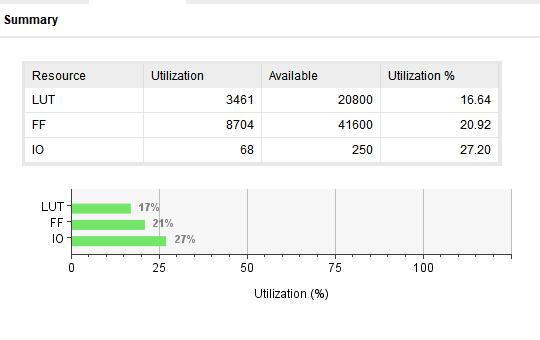
\includegraphics[scale=0.7]{sing.png}
    \caption{单周期处理器资源占用情况}
    \end{figure}

\subsection{CPI估算}
利用C语言程序将DataMemory.v中初始化的正整数列制作为二进制文件a.in,用于
运行汇编代码。测量排序算法部分的指令数:
\begin{figure}[H]
    \centering
    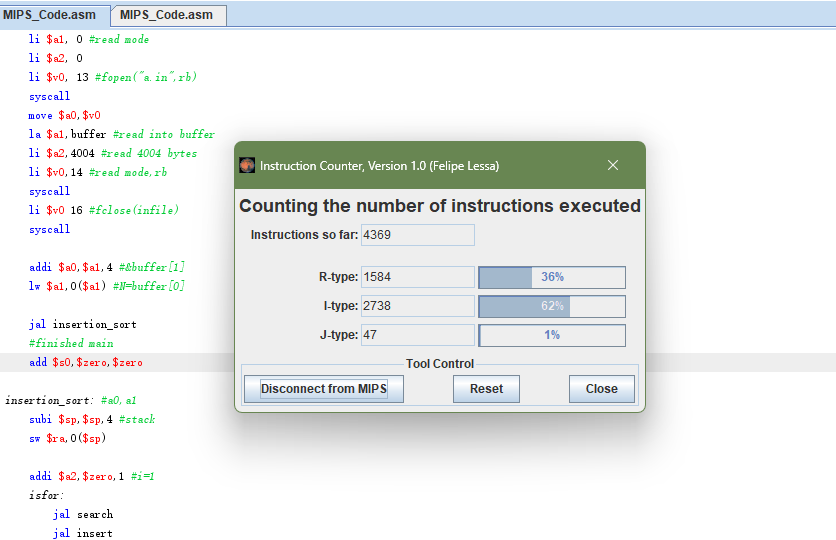
\includegraphics[scale=0.8]{clcc.png}
    \caption{排序算法指令数}
    \end{figure}
注意该测试代码的数据输入方式有所修改,经修正,排序算法指令数$I=4369-12=4357$
。

仿真测量排序算法部分的时钟周期数:
\begin{figure}[H]
    \centering
    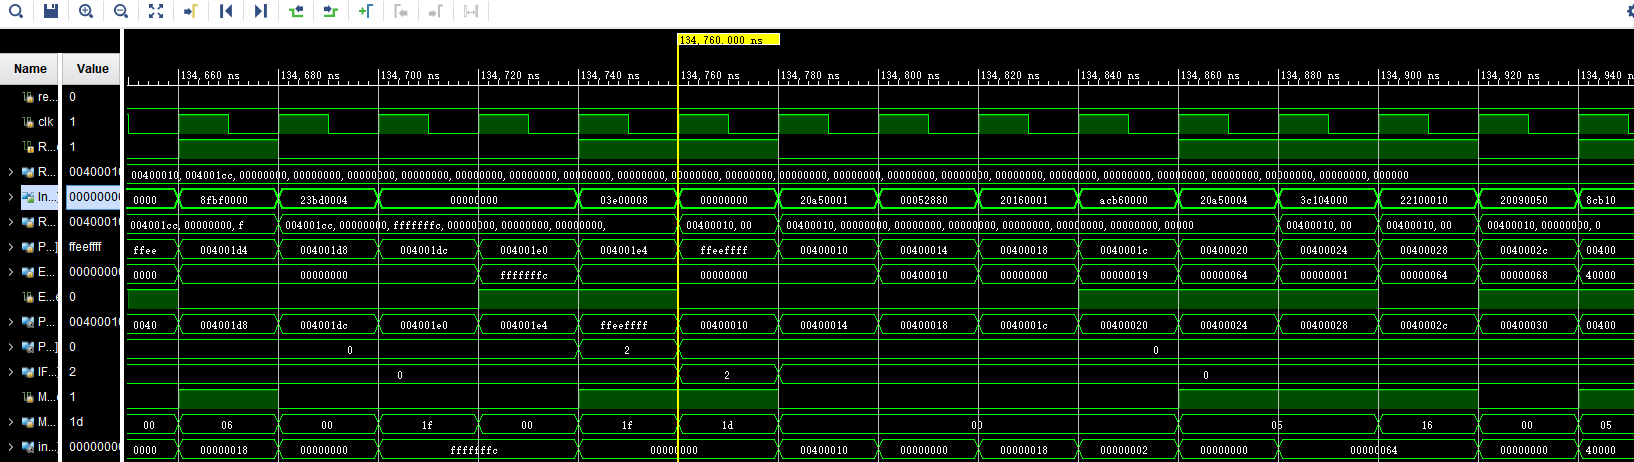
\includegraphics[scale=0.4]{clcs.png}
    \caption{排序算法运行周期数}
    \end{figure}
其中指令0x03e00008为排序算法部分的最后一条指令。此处已经经历的周期数为
$$C_0=\frac{134760ns}{20ns}=6738$$
故排序算法所需周期数为$C=C_0+4=6742$。

从而用该流水线处理器执行排序算法的$CPI=\frac{C}{I}\approx1.547$。
更换测试数据,CPI基本稳定在该值附近。CPI大于1的
主要缘故是Branch,Jump及其它冒险处理造成的阻塞。
\section{硬件调试情况}
在硬件调试(进行synthesis,implementation,generate bitstream)过程中遇到的主要问题,是
代码不规范引发的报错或板上行为异常,在behavioral simulation中不会观察到这些问题。
因此,仿真验证成功到上板显示成功还有一段路要走。

在DataMemory.v的设计中
——我曾使用两个always块初始化内存,这就产生了多驱动问题,致使implementation报错;在
RegisterFile.v中,我原使用always@(*)组合逻辑块,应用阻塞赋值实现寄存器先写后读,但
上板发现数码管与指示灯均不亮,代码运行可能出现死循环之类的问题。改用转发方式后,实验板
能够正常工作;在使用软件方式扫描显示数位时,我使用了接近MHz量级的扫描频率而非原本的1kHz——
一方面,汇编代码书写更简易,另一方面,频率较低时发现数码管有明显的闪烁问题。

此外,在硬件调试过程中还出现了其他问题,如端口位数不匹配等,这些问题并没有在behavioral simulation
的过程中被发现。我通过处理警告和报错一步步地解决了各种问题,最终完成了硬件调试,验收通过。

\begin{figure}[H]
    \centering
    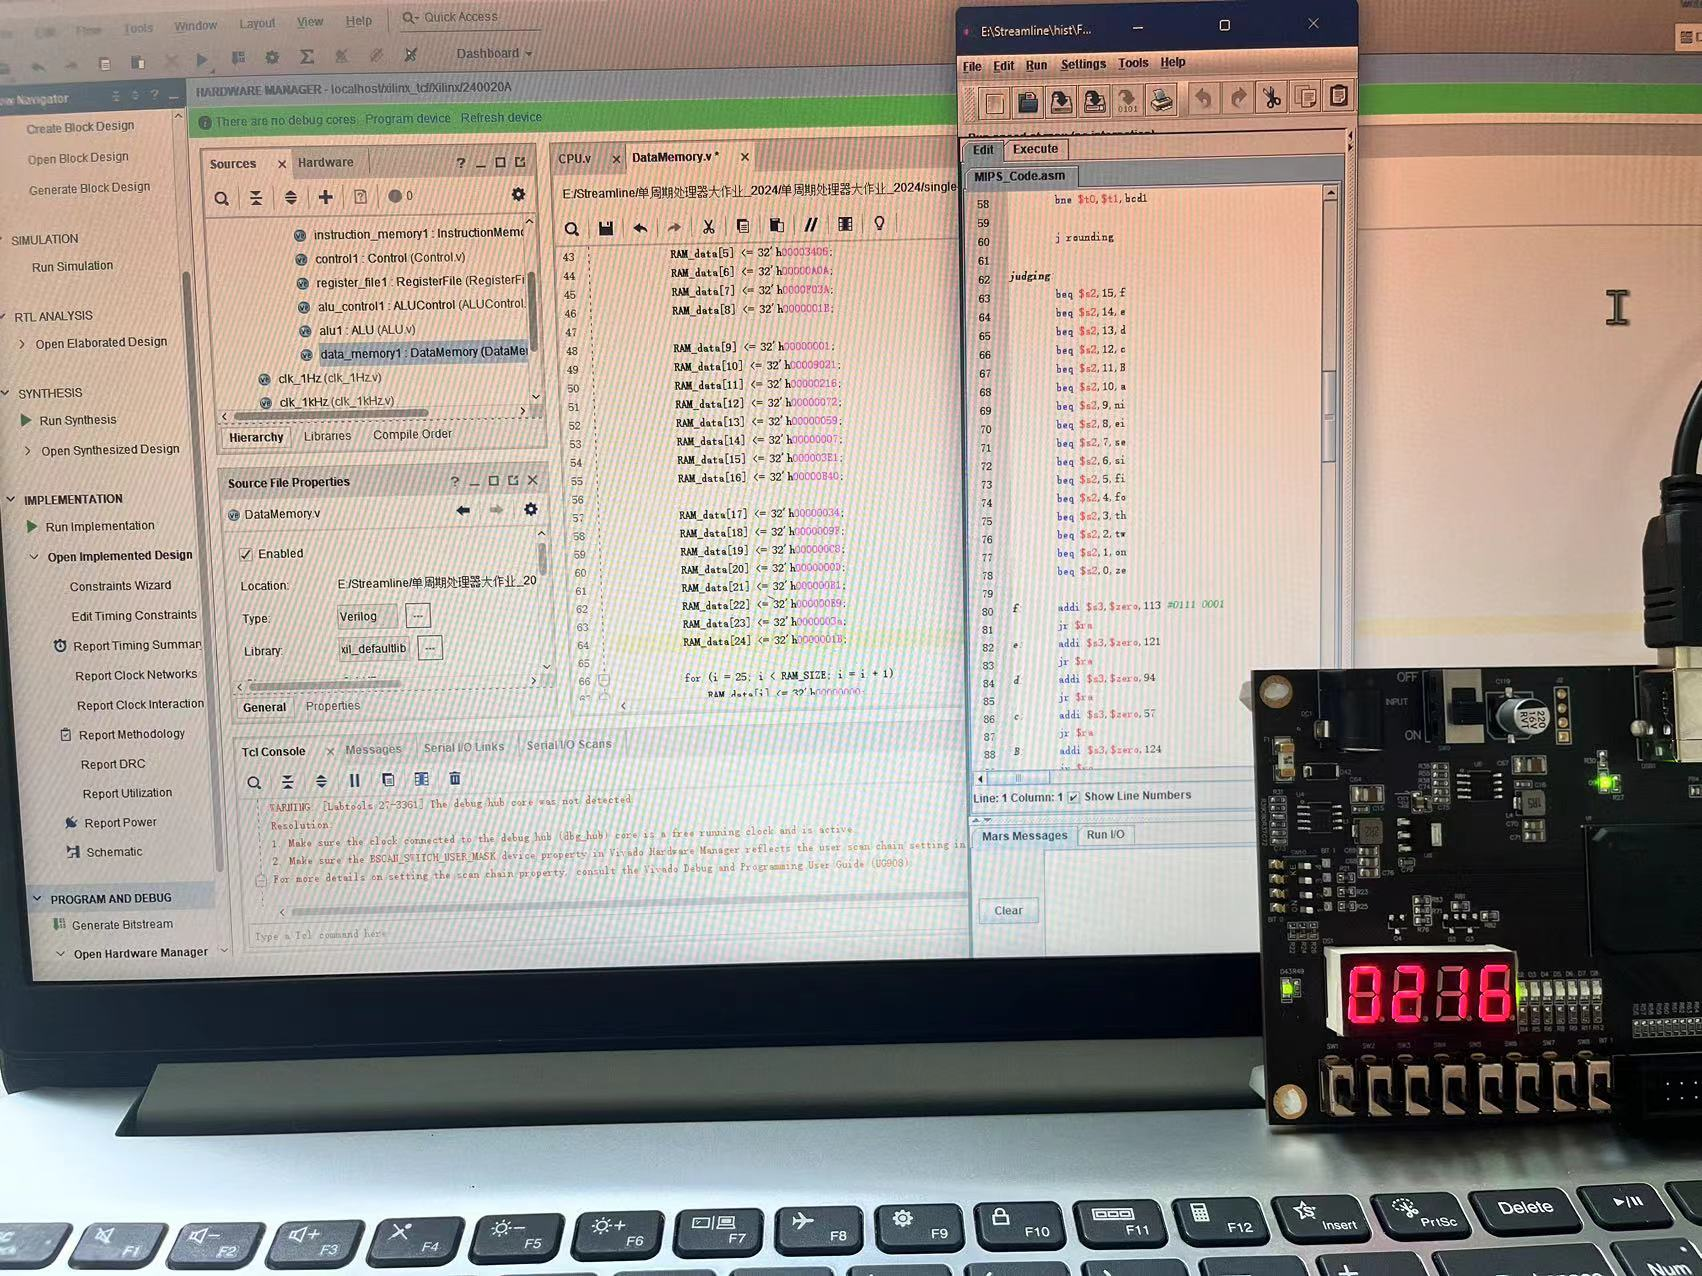
\includegraphics[scale=0.1]{k.jpg}
    \caption{硬件调试正常}
    \end{figure}
\section{思想体会}
本次实验使我收获颇丰,对我有非常深刻的影响。

我充分积累了编写大项目的宝贵经验——步步为营、循序渐进、勤加验证。处理器流水线化的过程,是添加功能的过程。
充分考虑应当实现的各种功能,相应地在程序上不断做加法即可。而只有做好规划,在功能实现上讲究一定的次序与逻辑,
才能尽量避免细节疏漏,避免千里之堤溃于蚁穴。在编写代码的过程中,我领悟并应用了
化整为零、逐个击破的技巧。在处理各种冒险时,
我遵循《数字逻辑与处理器基础》讲义,分别处理三类冒险,且同步进行
分开验证与合并验证,做到了全方位、无死角。我还认识到了备份及版本管理的重要性,遇到难以解决的bug时,
可以在邻近旧版本的基础上重新开始,一步步检查问题出现在哪一块新增代码上。频繁排查,遇到问题及时解决,
能够避免错误累积以至于积重难返。回想起来,如果没有上述“步步为营”“循序渐进”的习惯,
只需要一个bug,就可以让我迷失在庞大的代码块中,能不能按时完成任务都很成问题。

我充分培养了从事大工程所需要具备的良好品质——耐心谨慎、善于分析。本次流水线工程并非平地起高楼,而是
有单周期处理器的基础。这固然大大减轻了我编程的负担,但也考验着我的阅读分析能力。真正领会单周期处理器
代码的含义,是对之进行改造的前提。此外,耐心与分析能力是debug的必备品质。无论采用何种
聪明的编程战略,大小代码块产生问题都是难以避免的。要将汇编代码
(包含对应的机器语言)、verilog代码综合起来,结合仿真波形,不辞辛苦地全面分析。我曾一步步排查了近
百个时钟周期,尽管弄得眼睛疲劳、心情烦躁,终于锁定问题所在。解决问题之时,debug过程所带来的一切
折磨都换作了等量的轻松与喜悦。

本次实验全程由我独立完成。如果多加咨询老师助教、与他人多加交流参照,我的效率想必会更高,这是我应当反思改进的。然而,
独立实验的难度更大,也更能大大锻炼我解决问题的能力、促使我形成更独立深切的思想体会。在此,我要感谢
《数字逻辑与处理器基础实验》课程,在夏季学期为我提供了这样一次全面锻炼的机会!



\end{document}